% ------------------------------------------------------------- 
% Arquivo :  relatório modelo                                        
% ------------------------------------------------------------- 

\documentclass[brazilian,12pt,a4paper,final]{article}
% tamanhos de fontes: 10pt, 11pt ou 12pt
% opções de estilo (padrões): article, report, book, slide, letter (artigo, relatorio, livro, apresentação de slides, carta)
\usepackage[brazil]{babel}     % ifenização
%\usepackage{t1enc}            % reconhecimento dos acentos inseridos com o teclado
\usepackage[utf8]{inputenc}    %  reconhecimento dos caracteres com codificação UTF8, acentuação.
\usepackage{graphicx}          % figuras em formato eps 
%\usepackage[pdftex]{graphicx} % para produzir PDF diretamente
%\usepackage{color}             % fontes soloridas
\pdfimageresolution96
%%% fim do cabecalho %%%

%\pagestyle{empty}
\title{Análise de dados medidos em um filamento de tungstênio}
\author{Aluno: Átila Leites Romero \\ Matrícula: 144679 \\ IF-UFRGS}

\begin{document}
\maketitle

\begin{abstract}
Este trabalho apresenta uma verificação experimental da teoria de radiação de corpo negro, 
utilizando uma montagem onde foi medida a radiação emitida por uma lâmpada de tungstênio 
em função da potência elétrica fornecida.
\end{abstract}

\section{Introdução}
Segundo a lei de Stefan-Boltzmann,
$$ R_{(T)}=\sigma T^4$$
onde $R$ é a potência total irradiada, $\sigma$ é uma constante 
e $T$ é a temperatura do corpo negro. 

Mas a emissividade de corpos reais é menor que a emissividade de um corpo negro ideal.
Por isso, para corpos reais, a equação é reescrita como 
$$ R_{(T)}=\varepsilon (T)\sigma T^4$$
onde $\varepsilon$ é um número menor que $1$ e representa a emissividade do corpo.

Em outra experiência, foi verificado que as expressões
$$r=r_0+r_1(T-T_0)+r_2(T-T_0)^2$$ 
e 
$$r=r_0(\frac{T}{T_0})^\gamma$$
fornecem uma boa descrição para a
relação entre resistência e temperatura do filamento de tungstênio.

A potência total dissipada por efeito Joule pode ser calculada por 
$$P=VI$$ 
Assumindo que a energia dissipada por condução e convecção varie linearmente 
com a temperatura, pode-se afirmar que 
$$P_D=D(T-T_0)$$

Já a potência dissipada por radiação pode ser descrita pela lei de Stefan-Boltzmann, 
logo 
$$P=P_D+P_S=D(T-T_0)+S(T^4-T_0^4)$$
onde 
$$S=\sigma A 4\pi\varepsilon$$.

Como $\sigma$ é muito pequeno, 
para baixas temperaturas a dissipação por condução e convecção prevalece e,
por isso, 
$$P\simeq D(T-T_0)$$ 
e 
$$(T-T_0)\simeq \frac{P}{D}$$
o que leva a 
$$r=r_0+r_1\frac{P}{D}+r_2(\frac{P}{D})^2$$

Para altas temperaturas, a potência irradiada passa a prevalecer, 
já que cresce muito mais rápido que a potência dissipada por difusão térmica.
Neste caso,  
$$P\simeq S(T^4-T_0^4)$$ 
e, como 
$$T^4>>T_0^4$$, 
$$T^4\simeq \frac{P}{S}$$
o que leva a 
$$r=r_0\frac{1}{T_0^\gamma}(\frac{P}{S})^\frac{\gamma}{4}$$

Espera-se ainda que os dados experimentais possam ser descritos pela Lei de Planck
para radiação de corpo negro:
\[
R d\lambda=\frac{hc^2}{\lambda^5}\frac{1}{e^\frac{hc}{\lambda KT}-1} d\lambda
\]
Com a aproximação de Wien, $e^\frac{hc}{\lambda KT}-1$ é substituido 
por $e^\frac{hc}{\lambda KT}$ :
\[
R d\lambda=\frac{hc^2}{\lambda^5}e^\frac{-hc}{\lambda KT} d\lambda
\]

\section{Procedimento experimental}
Uma lâmpada de tungstênio com 20W de potência nominal foi ligada a uma fonte regulável. 
Um sensor fotoelétrico foi instalado em frente à lâmpada e ligado a um amplificador de tensão.

Foram aplicadas diferentes tensões à lâmpada.
Em cada etapa, eram medidas a corrente na lâmpada e a tensão de saída no sensor fotoelétrico, já amplificada.
Assumiu-se que a luminância detectada seria proprocional a esta tensão de saída, mesmo sendo desconhecido o valor exato desta proporção.

Na segunda parte da experiência, foram realizadas medidas outros materiais, porém sem 
a medida da luminância: lâmpada de 60W, filamento de tubo de Perrin, filamento de uma válvula 5Y3, um resistor de alta potência e um núcle de pilha Rayovac.

\section{Análise dos dados}
Para cada medida, 
a resistência do material pode ser calculada 
através da lei de Ohm: 
$$ r=V/I$$ 
onde $r$ é a resistência, $V$ a voltagem e $I$ a corrente aplicada ao material. 

Para voltagens baixas, o material estará em baixas temperaturas,
e é esperado um comportamento polinomial entre a 
resistência elétrica e a potência dissipada, descritas por
$$r=r_0+r_1\frac{P}{D}+r_2(\frac{P}{D})^2$$

Os valores para $r_0$, $\frac{r_1}{D}$ e $\frac{r_2}{D^2}$
podem ser calculados
utilizando regressão polinomial.

Para voltagens mais elevadas, se o filamento começar a irradiar, 
será esperado um crescimento geométrico da 
potência irradiada em relação à resistência, descrito por
$$r=r_0\frac{1}{T_0^\gamma}(\frac{P}{S})^\frac{\gamma}{4}$$

Neste caso a potência dissipada pode ser obtida a partir dos dados da luminosidade captada
pelo sensor fotoelétrico, no caso da lâmpada de 20W.

Para os outros materiais, que não tiveram a luminosidade medida, utiliza-se a potência fornecida, mas com o cuidado de
desconsiderar a parte dos dados onde a irradiação não predomina.
Para os materiais que não apresentarem irradiação predominante, não é calculado o $\gamma$.

Rearranjando os termos para isolar as constantes, temos:
$$\frac{r}{r_0}=(\frac{1}{T_0S^\frac{1}{4}}P^\frac{1}{4})^\gamma$$

E usando logaritmos:
$$ln(\frac{r}{r_0})=\gamma[ln(\frac{1}{T_0S^\frac{1}{4}})+ln(P^\frac{1}{4})]$$
$$ln(\frac{r}{r_0})=\gamma ln(\frac{1}{T_0S^\frac{1}{4}})+\frac{\gamma}{4}ln(P)$$
$$ln(\frac{r}{r_0})=A+Bln(P)$$
onde
$$A=\gamma ln(\frac{1}{T_0S^\frac{1}{4}}); B=\frac{\gamma}{4}$$


Os valores para $\gamma ln(\frac{1}{T_0S^\frac{1}{4}})$
e $\frac{\gamma}{4}$ podem ser calculados utilizando regressão linear.

Para o valor de $r_0$ da relação $\frac{r}{r_0}$, utiliza-se o valor obtido 
nas baixas voltagens.

Utilizando logaritmos com a aproximação de Wien, espera-se que 
o gráfico de ln(L)x$\frac{1}{T}$ produza uma reta com inclinação 
$-\frac{hc}{\lambda K}$:
\[
ln(L) =C-\frac{hc}{\lambda KT}
\]

Para calcular T, usa-se:
$$T=T_0(\frac{r}{r_0})^{1/\gamma}$$

Pode-se corrigir o cálculo da temperatura considerando a dilatação do material utilizando:
$$T_{corrigida}=T_0(\frac{r}{r_0})^{1/\gamma}(\frac{1+2\alpha(T_{ini}-T_0)}{1+\alpha(T_{ini}-T_0)})^{1/\gamma}$$

No entanto o erro introduzido por não utilizar esta correção é pequeno, em torno de 1\%.

Utilizando a inclinação $\beta$ da reta, pode-se calcular a constante de Planck
através de 
\[
h=-\beta \frac{\lambda K}{c}=-\beta \times 2.74705044 \times 10^{-19}
\]

\section{Lâmpada de 20W - primeiro conjunto de medidas}

No primeiro conjunto de dados 
não houve detecção de radiação luminosa até a voltagem de 1,1 volts.
Ou seja, até 1,1 volts, prevaleceu a difusão térmica.
Os valores calculados por regressão polinomial foram:
$$r_0=0,8148; \frac{r_1}{D}=3,820; \frac{r_2}{D^2}=-1,882$$

Na faixa de voltagens acima de 2 volts, foi notado um grande aumento da
potência dissipada, correspondente à dissipação por irradiação.

Os valores calculados por regressão linear foram:
$$\gamma ln(\frac{1}{T_0S^\frac{1}{4}}) = 1.286$$
$$\frac{\gamma}{4}=0,2963$$
$$\beta = -11284,6$$

Na figura \ref{figiniciopeq}, a regressão poninomial obtida utilizando 
valores até 1,1 volts é exibida.
Também é 
mostrado como seria o resultado nesta faixa caso todo o conjunto de dados fosse utilizado.

\begin{figure}[htbp!]
  \caption{Regressão polinomial para valores até 1,1 volts. Primeiro conjunto de medidas.}
  \label{figiniciopeq}
  \centering
    %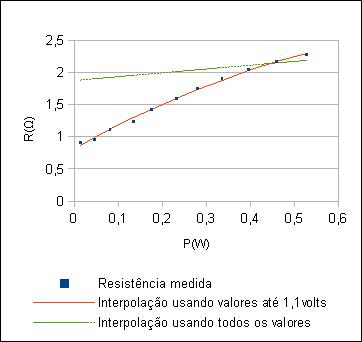
\includegraphics[scale=0.75]{iniciopeq.jpg}
    \resizebox{8.0cm}{!}{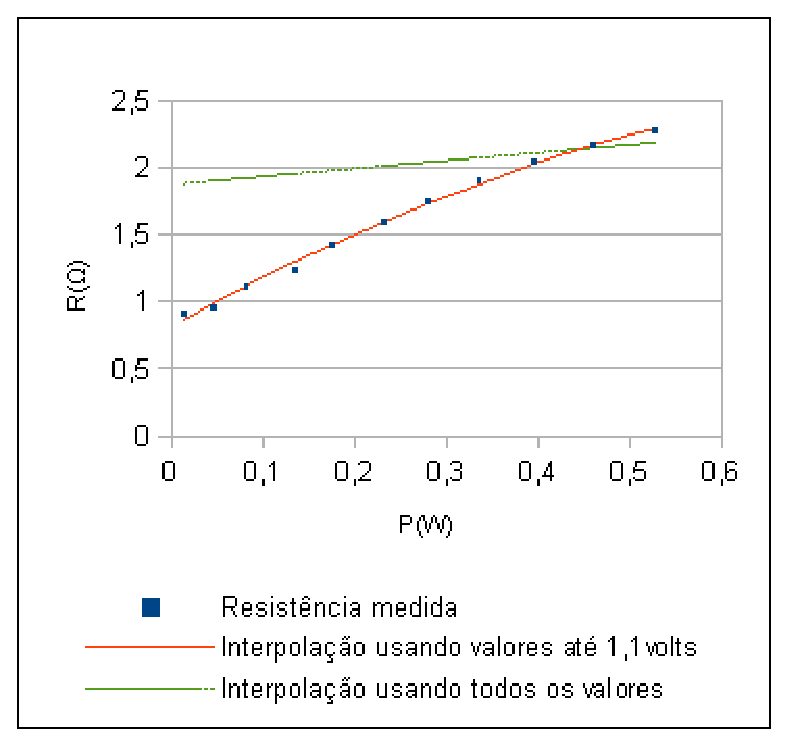
\includegraphics{iniciopeq.eps}}
\end{figure}

Na figura \ref{figfimpeq}, a regressão linear obtida utilizando 
os valores medidos a partir de 2 volts é exibida.

\begin{figure}[htbp!]
  \caption{Regressão linar para os logaritmos dos valores medidos a partir de 2 volts. Primeiro conjunto de medidas.}
  \label{figfimpeq}
  \centering
    %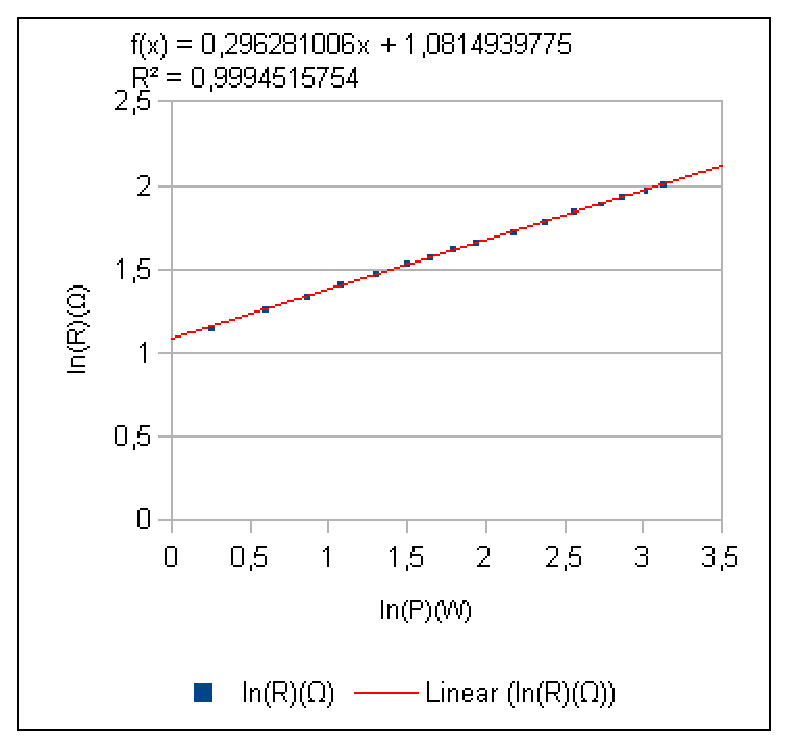
\includegraphics{fimpeq.eps}
    %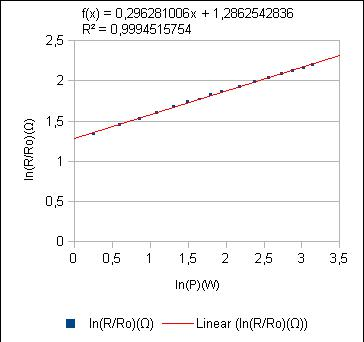
\includegraphics[scale=0.75]{fimpeq.jpg}
    \resizebox{8.0cm}{!}{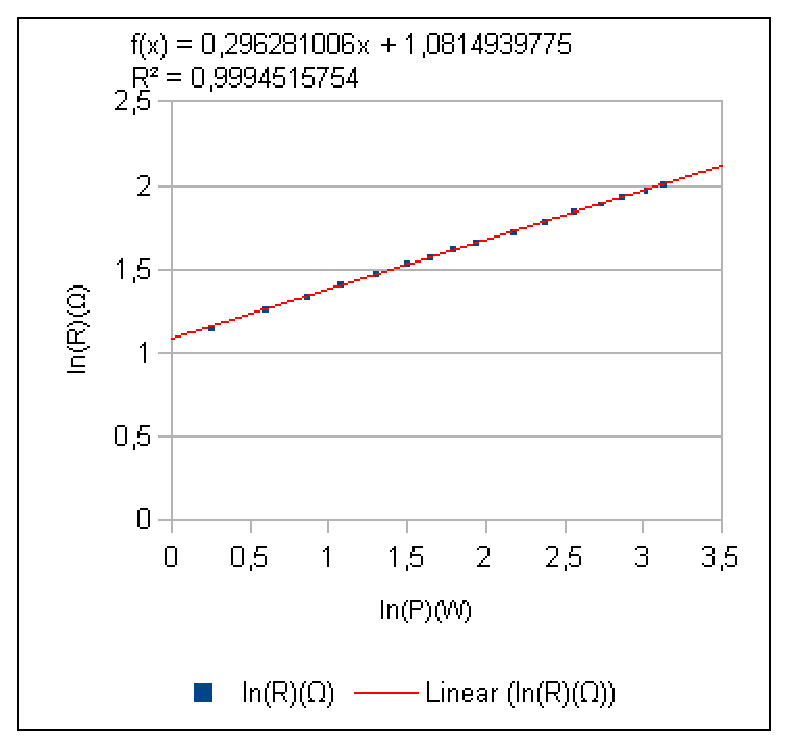
\includegraphics{fimpeq.eps}}
\end{figure}

Calculando $\gamma$ temos que:
$$\gamma=4\times 0,2963=1.185$$
que é próximo ao valor $1.221$ obtido em experiência prévia,
mas o material lá utilizado pode ter características diferentes,
como densidade e impurezas, que podem explicar parte desta diferença.


Na figura \ref{fighum}, foram comparados luminosidade e temperatura.
A regressão linear obtida informa a inclinação $\beta$, usada para o cálculo de $h$.

\begin{figure}[htbp!]
  \caption{Regressão linear do logaritmo da luminosidade versus 1/T. Primeiro conjunto de medidas.}
  \label{fighum}
  \centering
    %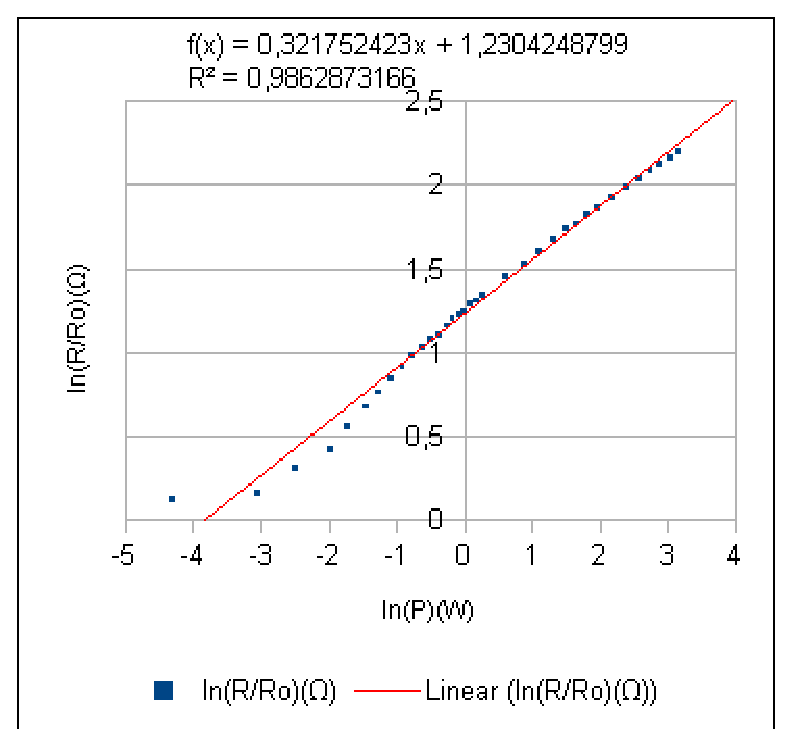
\includegraphics{fimgr.eps}
    %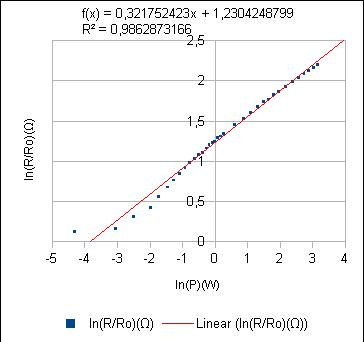
\includegraphics[scale=0.75]{fimgr.jpg}
    \resizebox{8.0cm}{!}{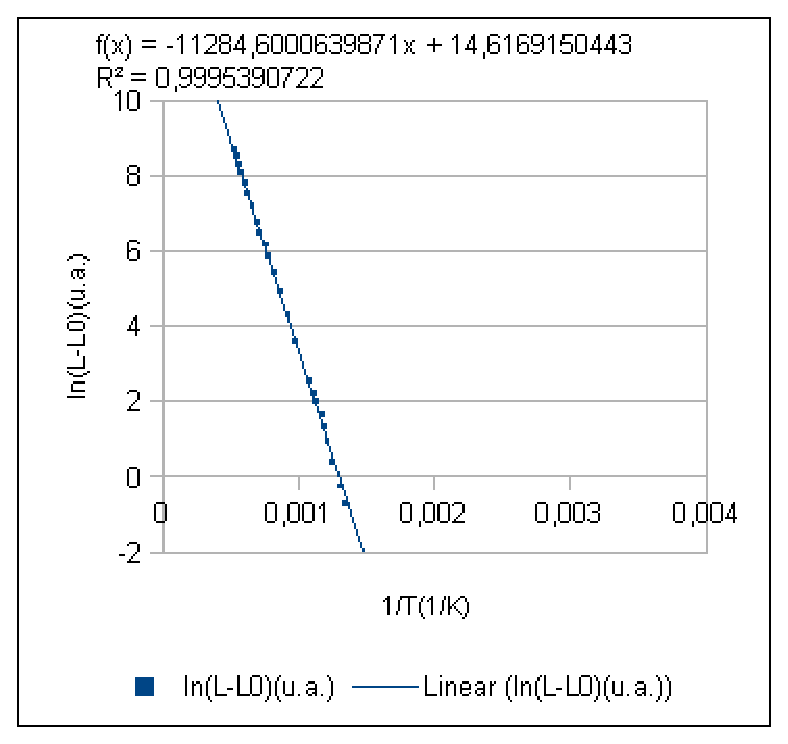
\includegraphics{h1.eps}}
\end{figure}

O valor calculado para $h$ foi $3.09993654 \times 10^{-15} eV.s$, que apresenta
um erro de aproximadamente 25\% em relação ao valor atualmente conhecido.

É possível que um número maior de medidas em baixas voltagens fornecesse
um valor mais preciso para $r_0$, o que aumentaria a precisão do $\gamma$
calculado.

Outra fonte de erro foi a luz da sala, que estava ligada durante o 
experimento, de modo que a movimentação das pessoas pode ter influenciado
a quantidade de luz incidente no sensor, 
alterando o resultado das medidas, sobretudo nas voltagens mais baixas.

Mesmo com essas aproximações, 
foi possível observar que a potência irradiada de fato aumentou
com a quarta potência da temperatura, 
o que está de acordo com a lei de Stefan-Boltzmann.

\section{Lâmpada de 20W - segundo conjunto de medidas}

No segundo conjunto de dados, 
não houve detecção de radiação luminosa até a voltagem de 0,650 volts.
Ou seja, até 0,650 volts, prevaleceu a difusão térmica.
Os valores calculados por regressão polinomial foram:
$$r_0=0,6543; \frac{r_1}{D}=3,762; \frac{r_2}{D^2}=-1,361$$

Na faixa de voltagens acima de 2,60 volts, foi notado um grande aumento da
potência dissipada, correspondente à dissipação por irradiação.

Os valores calculados por regressão linear foram:
$$\gamma ln(\frac{1}{T_0S^\frac{1}{4}}) = 1,481$$
$$\frac{\gamma}{4}=0,3002$$

Na figura \ref{figiniciopeq2}, a regressão poninomial do segundo conjunto
de dados, obtida utilizando 
valores de até 0,650 volts é exibida.

\begin{figure}[htbp!]
  \caption{Regressão polinomial para valores até 0,650 volts. Segundo conjunto de medidas.}
  \label{figiniciopeq2}
  \centering
    %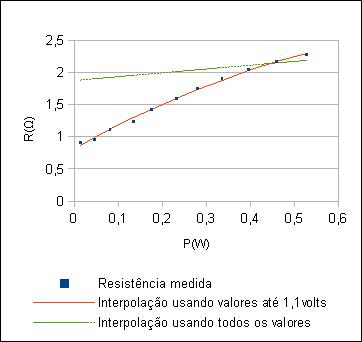
\includegraphics[scale=0.75]{iniciopeq.jpg}
    \resizebox{8.0cm}{!}{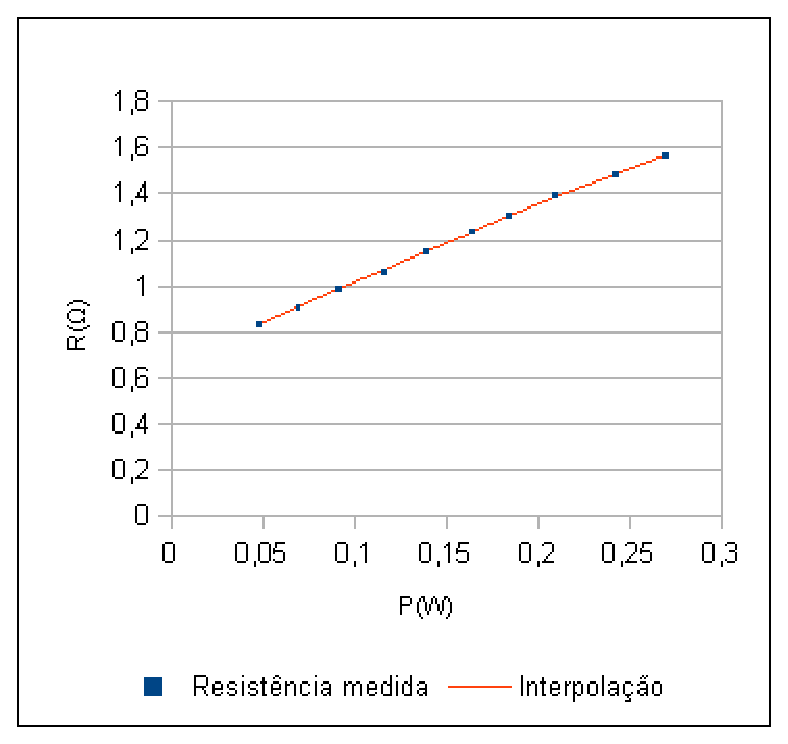
\includegraphics{iniciopeq2.eps}}
\end{figure}

Na figura \ref{figfimpeq2}, a regressão linear do segundo conjunto de dados, 
obtida utilizando os valores medidos a partir de 2,60 volts é exibida.

\begin{figure}[htbp!]
  \caption{Regressão linar para os logaritmos dos valores medidos a partir de 2,60 volts. Segundo conjunto de medidas.}
  \label{figfimpeq2}
  \centering
    %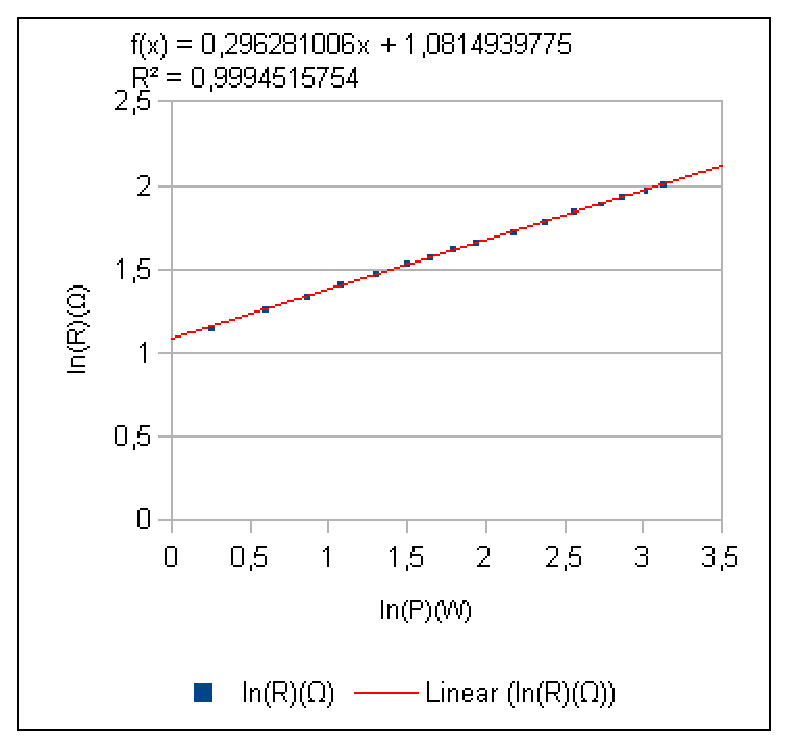
\includegraphics{fimpeq.eps}
    %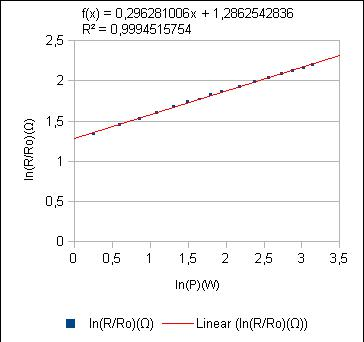
\includegraphics[scale=0.75]{fimpeq.jpg}
    \resizebox{8.0cm}{!}{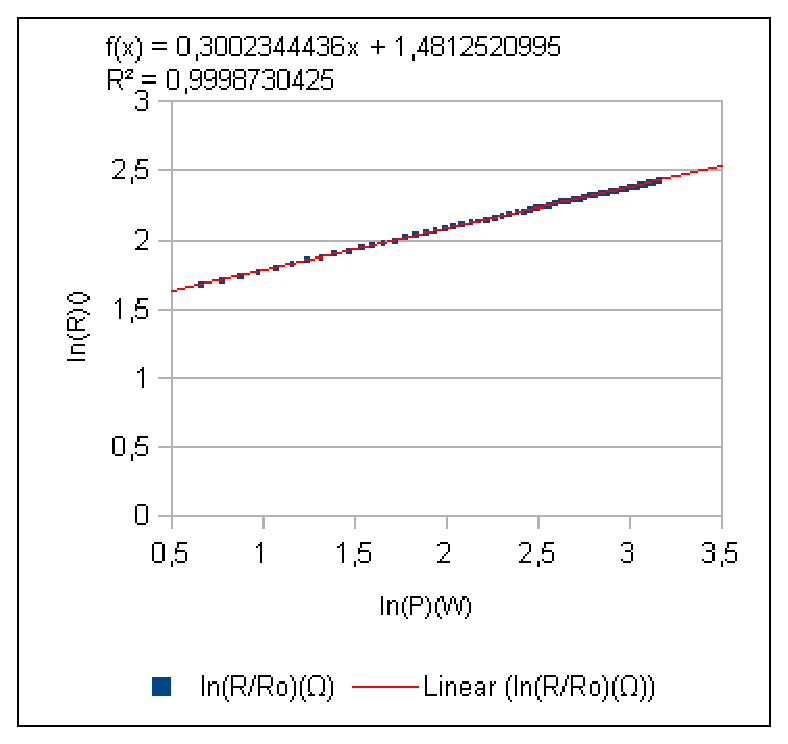
\includegraphics{fimpeq2.eps}}
\end{figure}

Calculando $\gamma$ temos que:
$$\gamma=4\times 0,3002=1,200$$
que é mais próximo ao valor $1.221$ obtido em experiência prévia que 
aquele obtido no primeiro conjunto de dados.

Na figura \ref{fighhh}, foram comparados luminosidade e temperatura. A regressão linear obtida informa a inclinação $\beta$, usada para o cálculo de $h$.

\begin{figure}[htbp!]
  \caption{Regressão linear do logaritmo da luminosidade versus 1/T. Segundo conjunto de medidas.}
  \label{fighhh}
  \centering
    %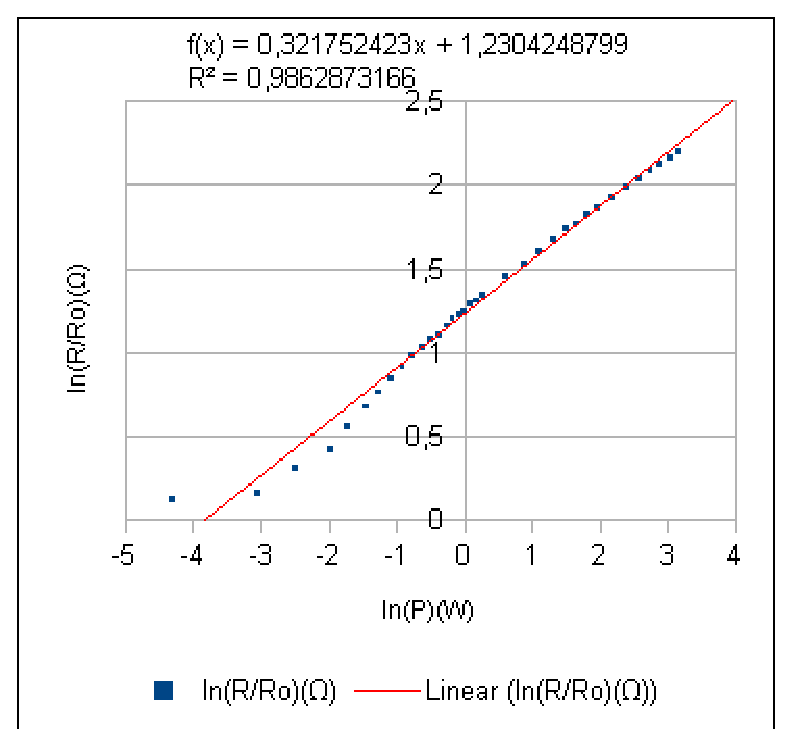
\includegraphics{fimgr.eps}
    %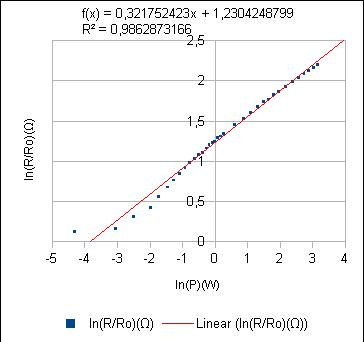
\includegraphics[scale=0.75]{fimgr.jpg}
    \resizebox{8.0cm}{!}{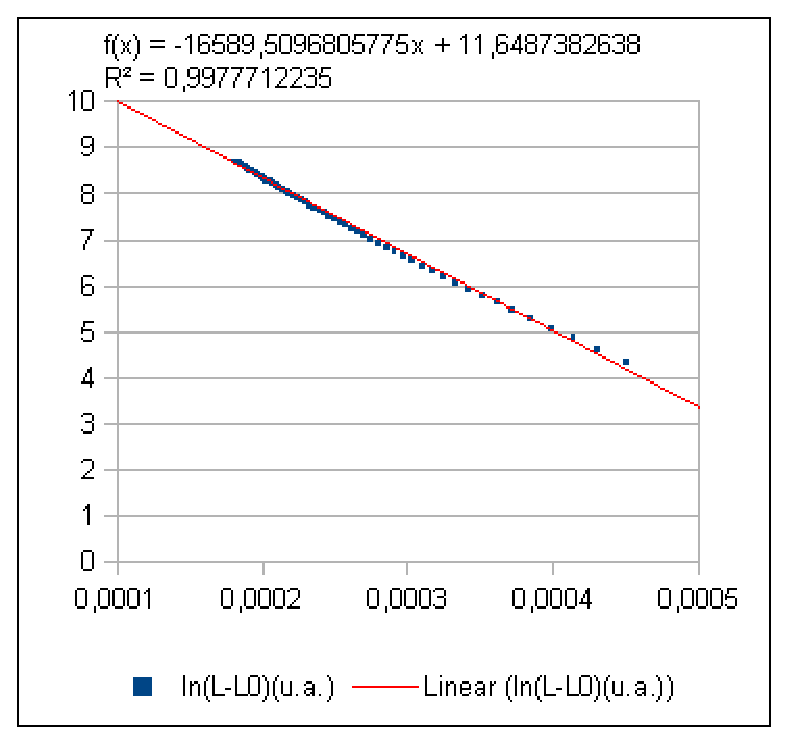
\includegraphics{h2.eps}}
\end{figure}

O valor calculado para $h$ foi $4.55721933 \times 10^{-15} eV.s$, que apresenta
um erro de aproximadamente 10\% em relação ao valor atualmente conhecido.

\section{Segunda parte - outros materiais}

Os dados medidos e os calculados na segunda parte da experiência podem ser
visualizados no gráfico \ref{rxptodos}. Algums materiais estão exibidos também
no gráfico \ref{rxpsel}, para melhor visualização.

\begin{figure}[htbp!]
  \caption{RxP - Dados medidos para diversos materiais.}
  \label{rxptodos}
  \centering
    %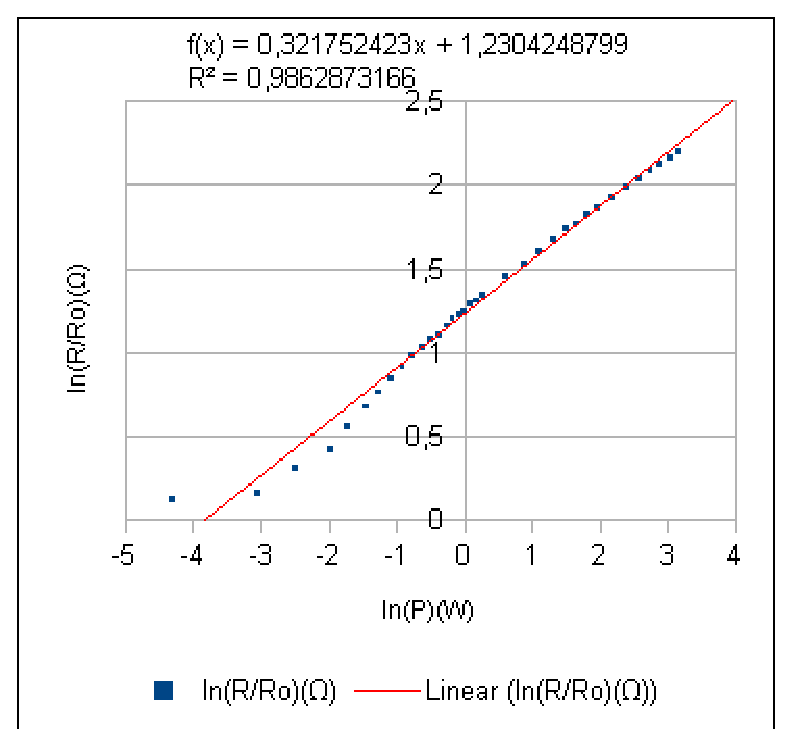
\includegraphics{fimgr.eps}
    %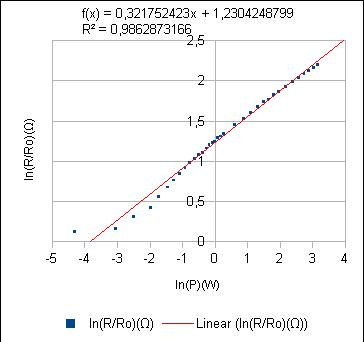
\includegraphics[scale=0.75]{fimgr.jpg}
    \resizebox{8.0cm}{!}{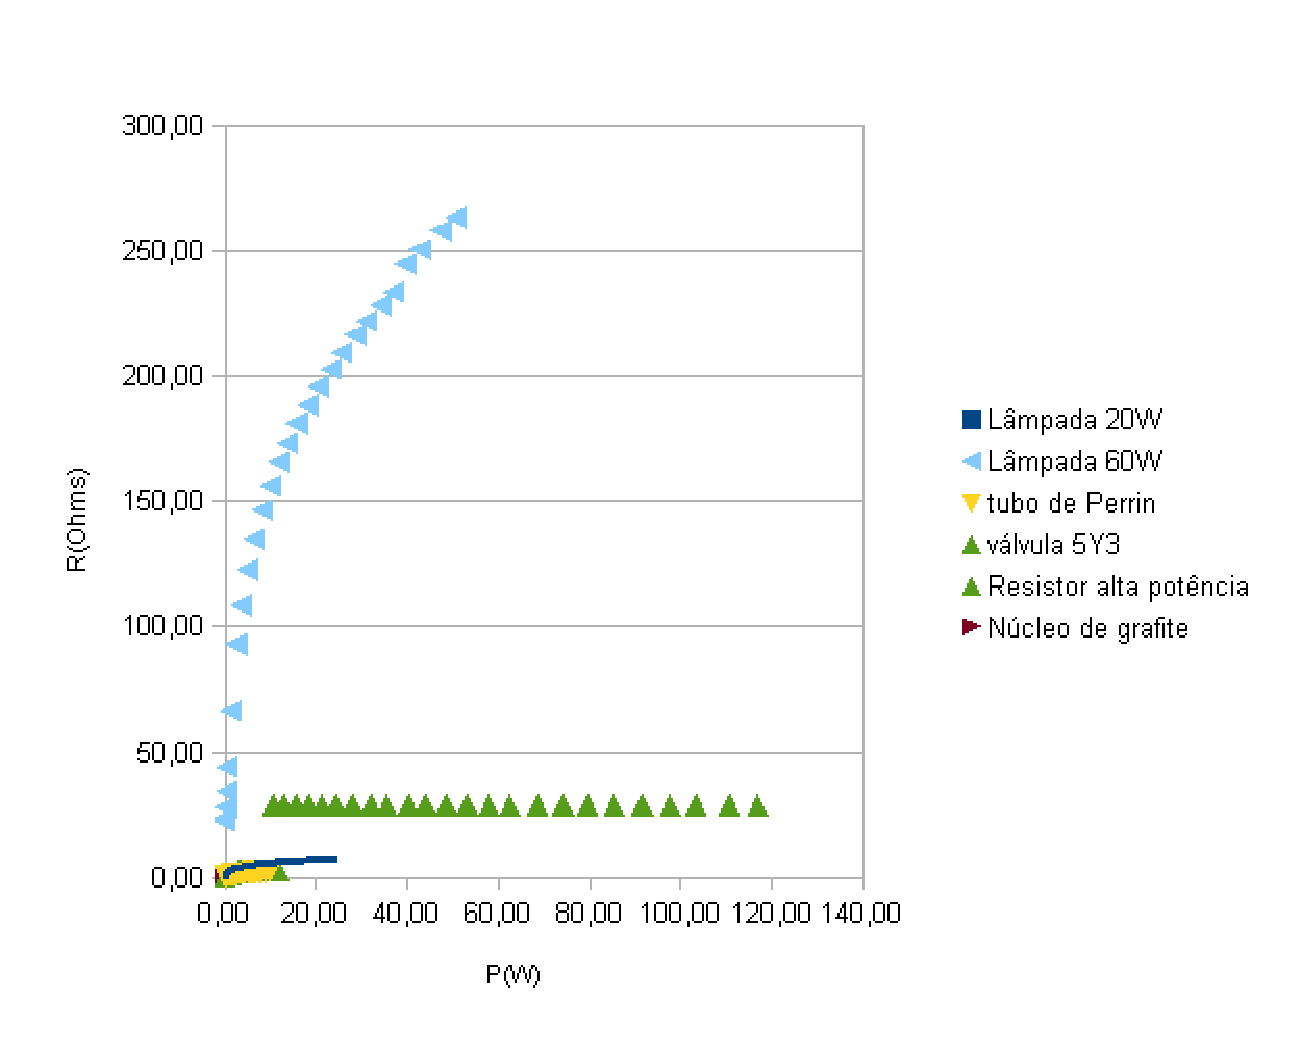
\includegraphics{rxptodos.eps}}
\end{figure}

\begin{figure}[htbp!]
  \caption{RxP - Dados medidos para diversos materiais.}
  \label{rxpsel}
  \centering
    %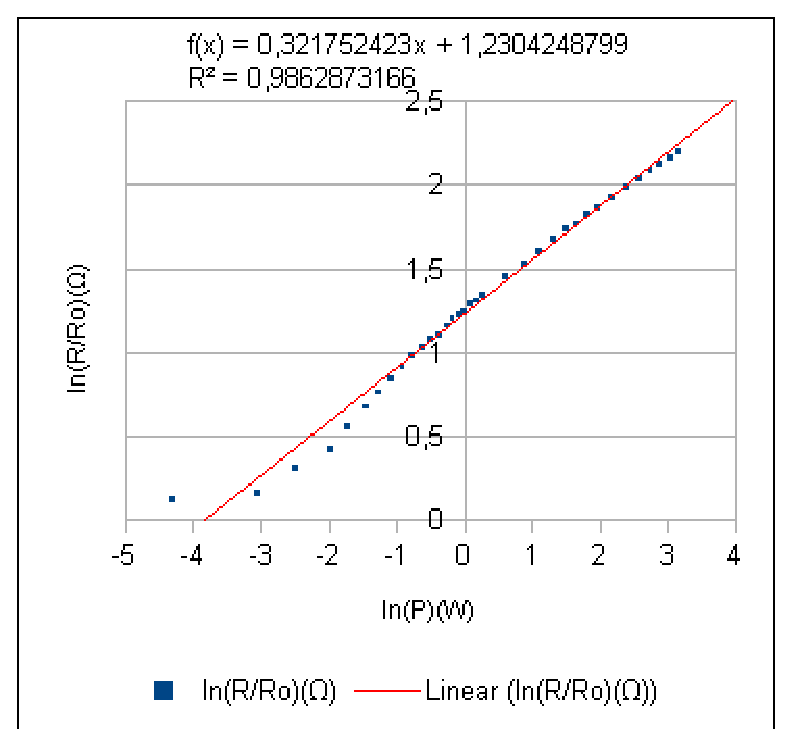
\includegraphics{fimgr.eps}
    %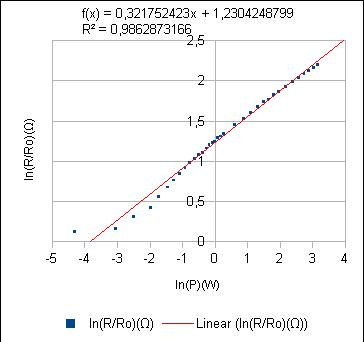
\includegraphics[scale=0.75]{fimgr.jpg}
    \resizebox{8.0cm}{!}{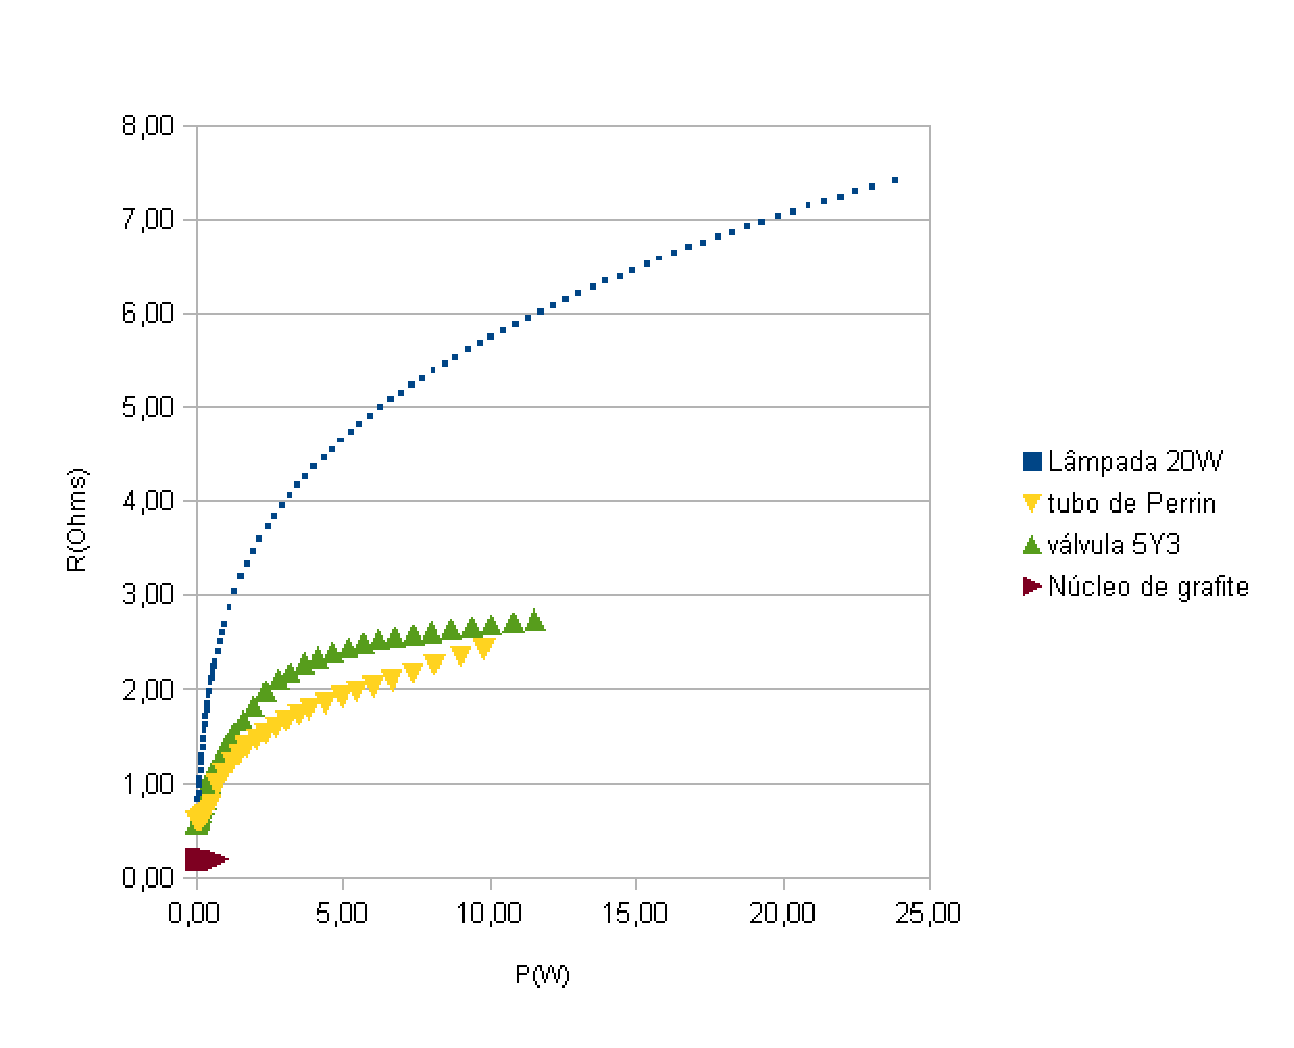
\includegraphics{rxpsel.eps}}
\end{figure}

Os valores obtidos para $r_0$ foram:

lâmpada de 60W: 21,88 Ohms

tubo de Perrin: 0,59 Ohms

válvula 5Y3: 0,55 Ohms

resistor de alta potência: 28,71 Ohms

núcleo de pilha - grafite: 0,19 Ohms

Os valores obtidos para $\gamma$ foram:

lâmpada de 60W: 1,32

tubo de Perrin: 1,27

válvula 5Y3: 0,76

A lâmpada de 60W e 
o tubo de Perrin parecem ser de tungstênio.
A válvula 5Y3 parece não ser predominantemente de tungstênio, ou a dissipação por
difusão térmica ainda era considerável.
A diferença pode ser observada no gráfico \ref{gamma}, pela inclinação das retas.

\begin{figure}[htbp!]
  \caption{ln(R/R0)xln(P) - Uso da inclinação das retas para o cálculo de gama.}
  \label{gamma}
  \centering
    %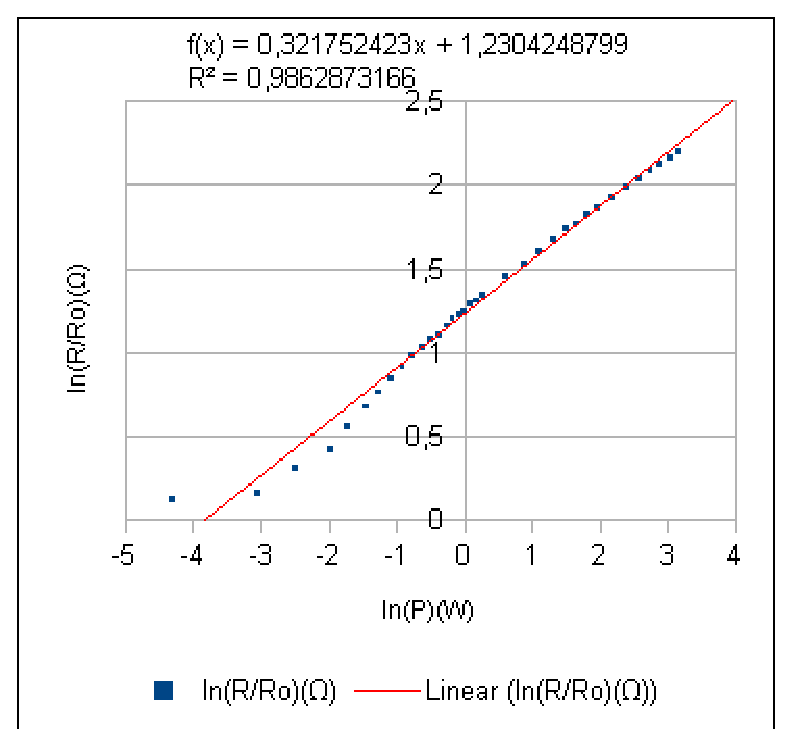
\includegraphics{fimgr.eps}
    %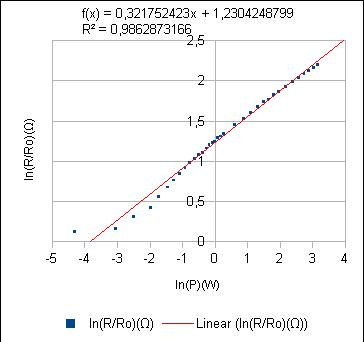
\includegraphics[scale=0.75]{fimgr.jpg}
    \resizebox{8.0cm}{!}{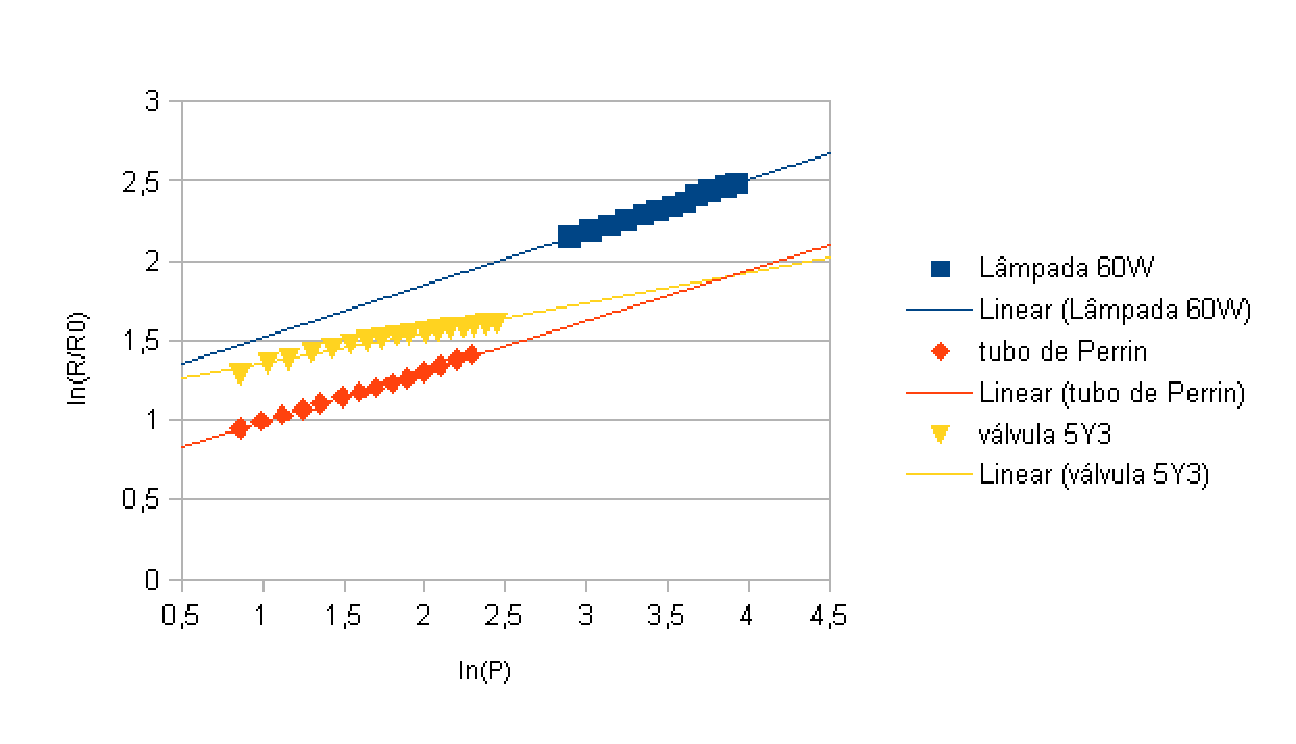
\includegraphics{gamma.eps}}
\end{figure}

O resistor de alta potência e o núcleo de pilha não apresentaram 
predominância de irradiação e, portanto, não foi possível calcular o $\gamma$ 
para estes materiais.

Comparando $P$ e $T^4$ no gráfico \ref{t4}, pode-se notar que para a lâmpada de 60W e para o filamento do tubo de Perrin, existe uma correspondência linear entre $P$ e $T^4$, o que está de acordo com a lei de Stefan-Boltzmann. Já para a válvula, nota-se que a dissipação ainda é de fato significativa, já que não produziu uma reta. Este fato deve ter alterado o valor de gama para este material e, portanto dificulta que seja definida uma conclusão categórica para sua composição.

\begin{figure}[htbp!]
  \caption{$T^4$x$P$ - Confirmação da lei de Stefan-Boltzmann.}
  \label{t4}
  \centering
    %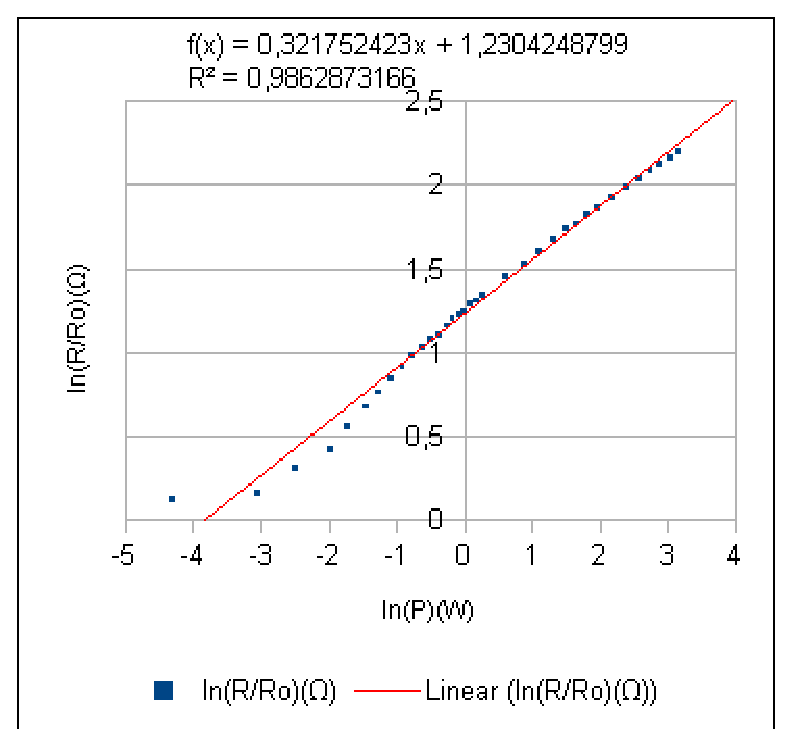
\includegraphics{fimgr.eps}
    %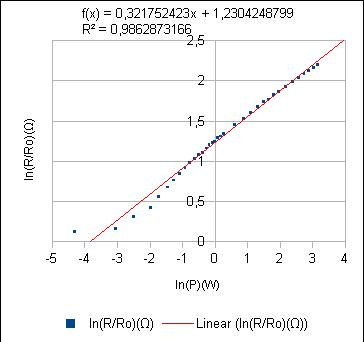
\includegraphics[scale=0.75]{fimgr.jpg}
    \resizebox{8.0cm}{!}{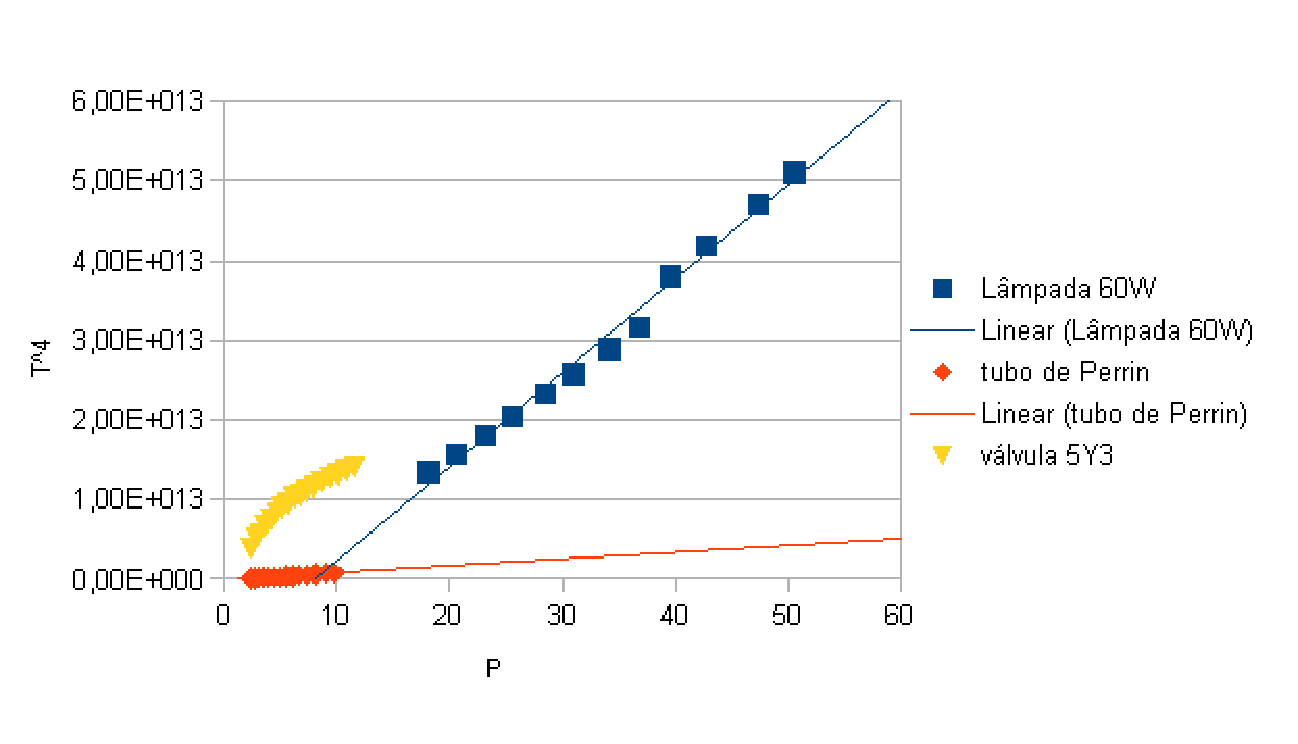
\includegraphics{t4.eps}}
\end{figure}

\section{Conclusões}
Neste experimento medimos a potência dissipada por um filamento de tungstênio
sujeito a diferentes voltagens. Foi confirmado que a difusão térmica predomina
em baixas temperaturas e que a irradiação predomina em temperaturas maiores.

O modelo de dissipação de energia para baixas temperaturas
assume que a relação entre potência dissipada e temperatura é linear
e descreveu satisfatóriamente as medidas feitas em baixa voltagem.

Para altas temperaturas, 
o modelo que considera que 
a energia dissipada é proporcional à quarta potência da temperatura 
forneceu uma descrição mais adequada para as medidas obtidas.

Os valores calculados para a constante de Planck utilizando os dois conjuntos
de dados apresentaram aproximações razoáveis em relação aos valores atualmente
conhecidos, principalemente se for considerado que a constante é um número
muito pequeno, com uma ordem de grandeza -15.

O segundo conjunto de medidas apresentou resultados melhores do que o 
primeiro, por conter mais pontos na faixa de baixas voltagens e por 
apresentar uma precisão maior, que pode ser notada pela menor variação
de luminosidade nesta mesma faixa.

Na segunda parte da experiência foi interessante notar como a resistividade de 
diferentes materiais se comporta em relação a potência fornecida.


%\begin{thebibliography}{99}
%\end{thebibliography}

\end{document}

